
\section{Zulassung}
\label{section:zulassung}
\begin{frame}%STARTCONTENT

\frametitle{Zulassung}
\begin{itemize}
  \item Neben einer erfolgreich abgelegten Amateurfunkprüfung ist eine \enquote{Zulassung zur Teilnahme am Amateurfunkdienst} unbedingt erforderlich, damit man eine Amateurfunkstelle betreiben darf.
  \end{itemize}
\begin{itemize}
  \item Dieser Zulassung geht die Erteilung eines personengebundenen Rufzeichens einher.
  \end{itemize}
\begin{itemize}
  \item Das Amateurfunkgesetz (AFuG) sieht kein Mindestalter vor.
  \end{itemize}
\end{frame}

\begin{frame}
\begin{figure}
    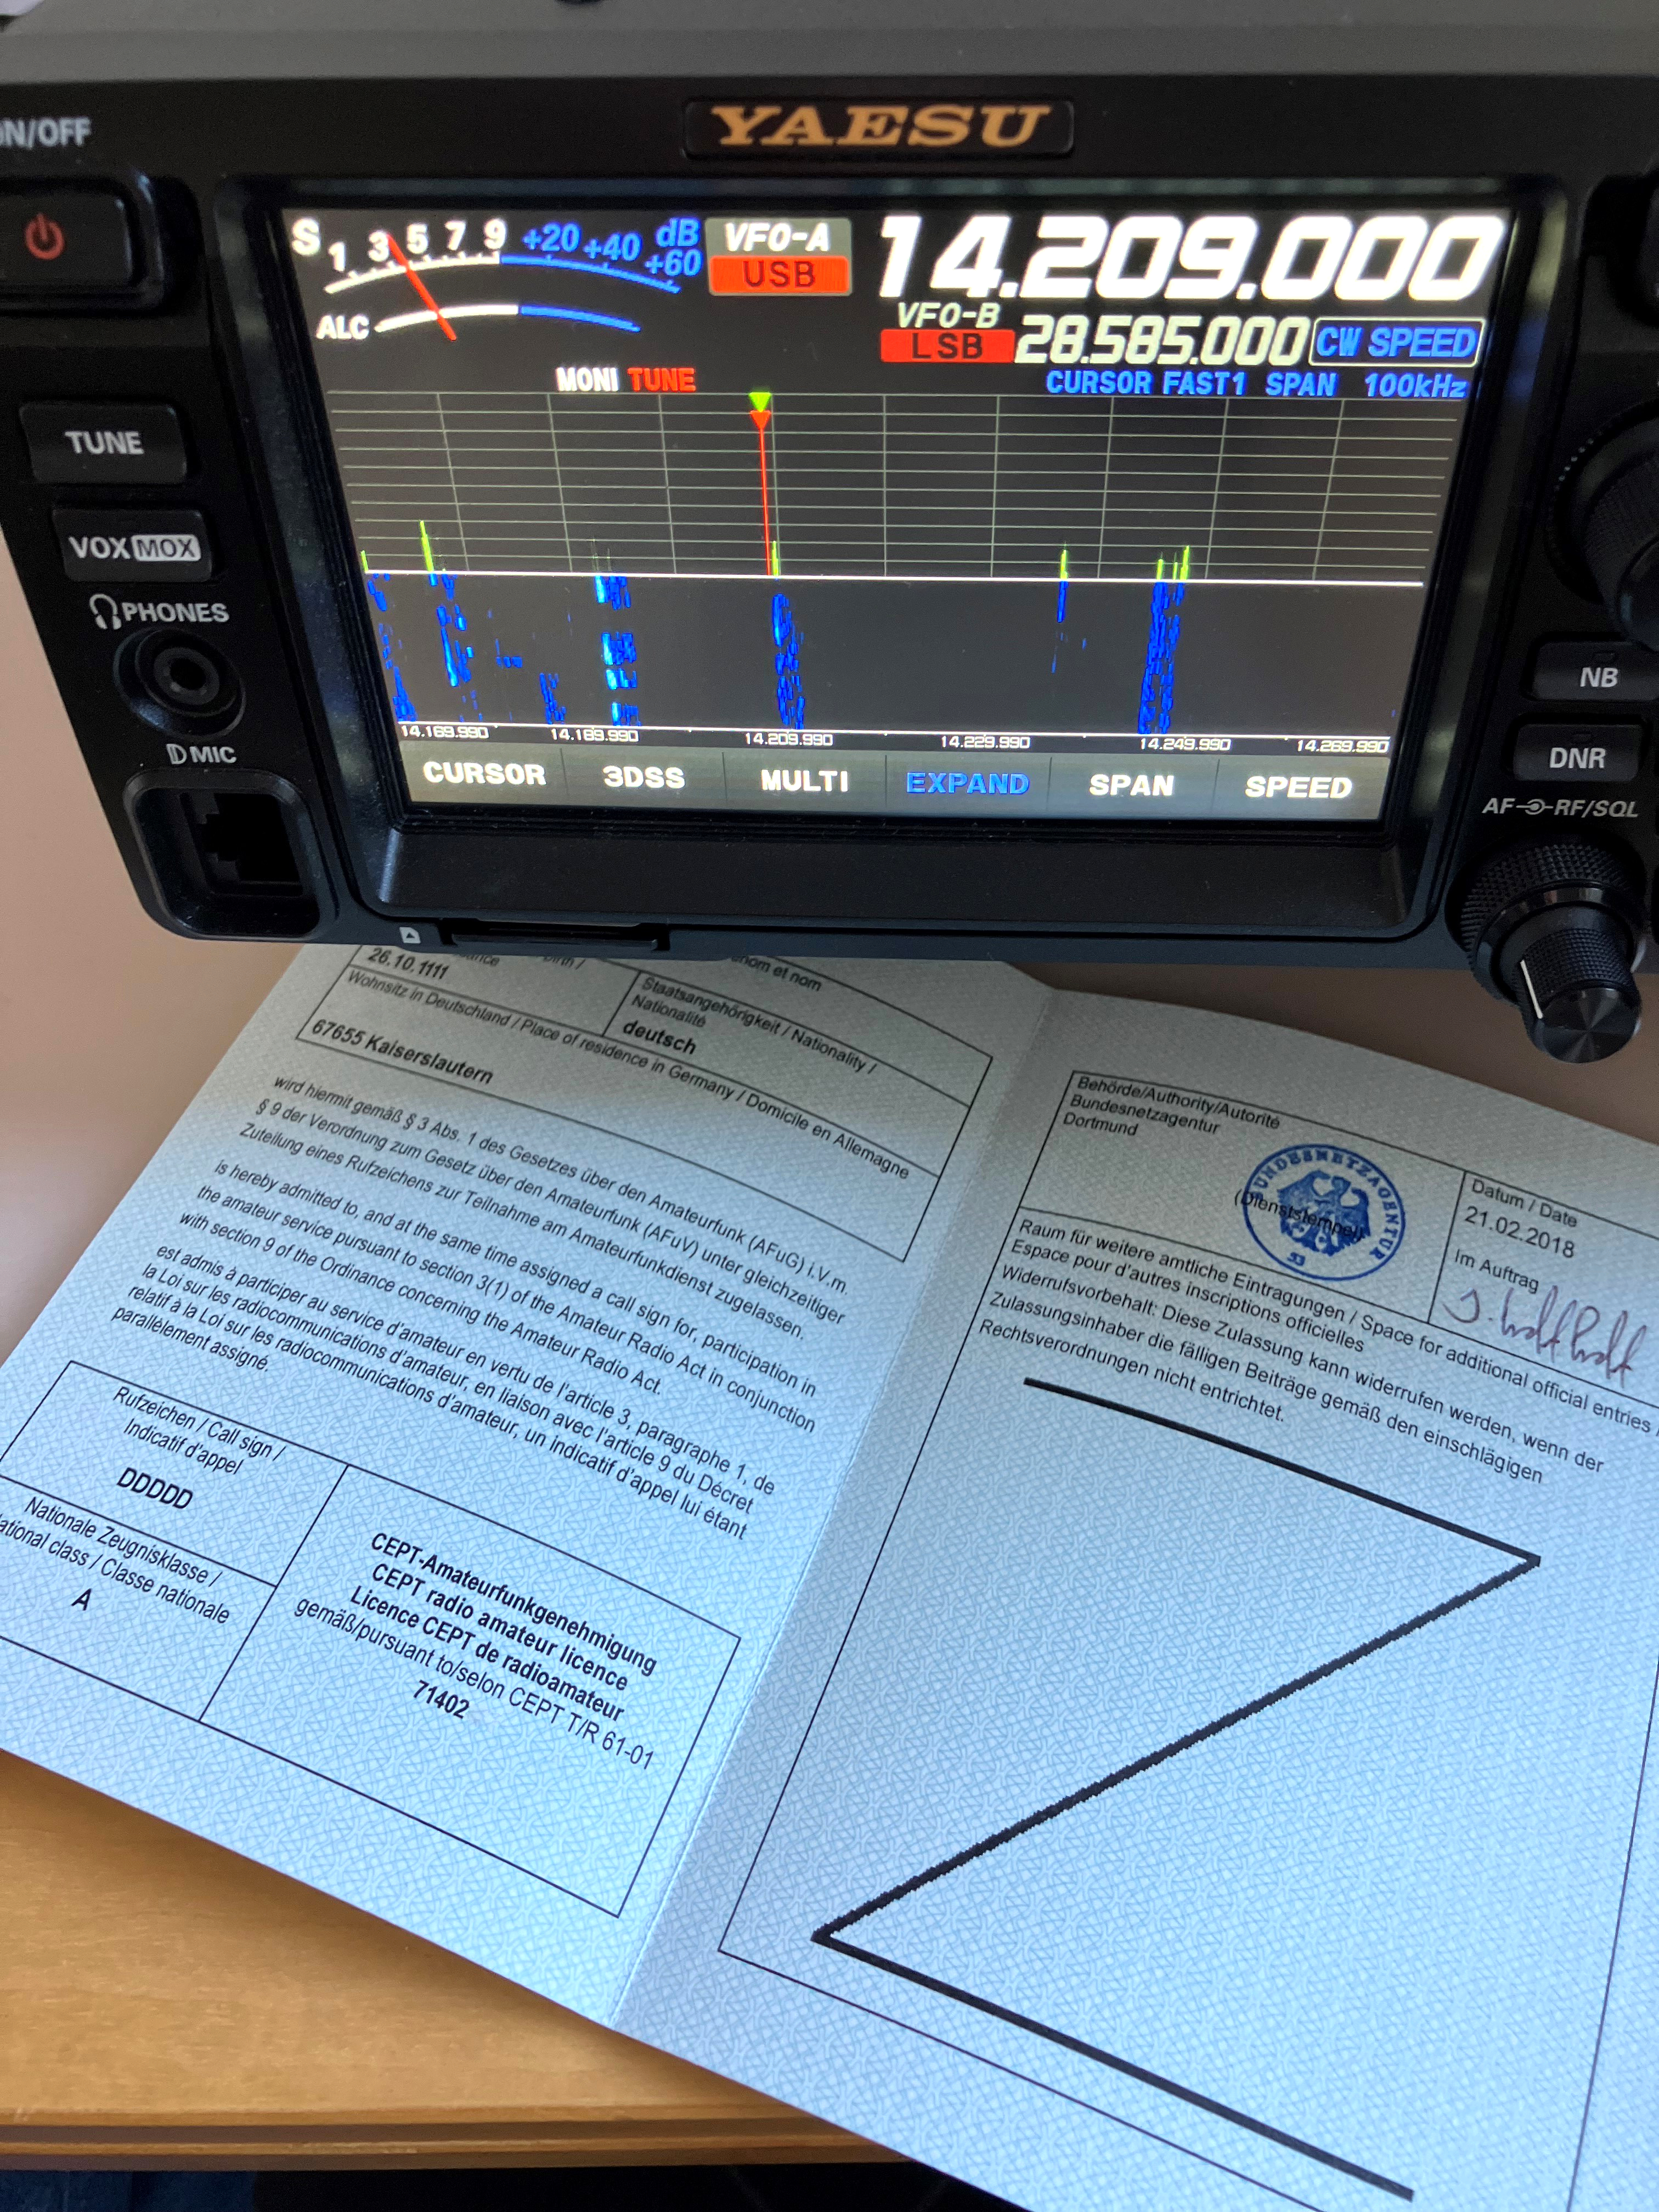
\includegraphics[width=0.85\textwidth]{foto/91}
    \caption{\scriptsize Die Zulassungsurkunde}
    \label{n_zulassung_urkunde}
\end{figure}
\end{frame}

\begin{frame}
\only<1>{
\begin{QQuestion}{VC106}{Was ist neben einer erfolgreich abgelegten Amateurfunkprüfung unbedingt erforderlich, damit Sie eine Amateurfunkstelle betreiben dürfen?}{Die Vorlage eines Nachweises über die fachgerechte Installation der Antennenanlage}
{Eine Zulassung zur Teilnahme am Amateurfunkdienst}
{Die Einholung einer EMVU-Bescheinigung von der zuständigen Behörde}
{Die Vorlage von Berechnungsunterlagen und ergänzenden Messprotokollen der ungünstigsten Konfiguration der Antennenanlage}
\end{QQuestion}

}
\only<2>{
\begin{QQuestion}{VC106}{Was ist neben einer erfolgreich abgelegten Amateurfunkprüfung unbedingt erforderlich, damit Sie eine Amateurfunkstelle betreiben dürfen?}{Die Vorlage eines Nachweises über die fachgerechte Installation der Antennenanlage}
{\textbf{\textcolor{DARCgreen}{Eine Zulassung zur Teilnahme am Amateurfunkdienst}}}
{Die Einholung einer EMVU-Bescheinigung von der zuständigen Behörde}
{Die Vorlage von Berechnungsunterlagen und ergänzenden Messprotokollen der ungünstigsten Konfiguration der Antennenanlage}
\end{QQuestion}

}
\end{frame}

\begin{frame}
\only<1>{
\begin{QQuestion}{VC108}{Ist nach dem Amateurfunkgesetz (AFuG) für die Erteilung einer Amateurfunkzulassung ein Mindestalter erforderlich?}{Für die Erteilung der Klasse A ist  die Volljährigkeit Voraussetzung.}
{Das Mindestalter für die Antragstellung beträgt 15~Jahre.}
{Das Amateurfunkgesetz (AFuG) sieht ab Klassen E ein Mindestalter von 16~Jahren vor.}
{Das Amateurfunkgesetz (AFuG) sieht kein Mindestalter vor.}
\end{QQuestion}

}
\only<2>{
\begin{QQuestion}{VC108}{Ist nach dem Amateurfunkgesetz (AFuG) für die Erteilung einer Amateurfunkzulassung ein Mindestalter erforderlich?}{Für die Erteilung der Klasse A ist  die Volljährigkeit Voraussetzung.}
{Das Mindestalter für die Antragstellung beträgt 15~Jahre.}
{Das Amateurfunkgesetz (AFuG) sieht ab Klassen E ein Mindestalter von 16~Jahren vor.}
{\textbf{\textcolor{DARCgreen}{Das Amateurfunkgesetz (AFuG) sieht kein Mindestalter vor.}}}
\end{QQuestion}

}
\end{frame}%ENDCONTENT
